\section*{Introduction}
Since images stored on computers are simply matrices where each element
represents a pixel, matrix methods learned in class can be used to
modify images. The purpose of this project was to apply matrix manipulations
on given image files, shown below as Figure~\ref{fig:p1} and
Figure~\ref{fig:p2}.

\begin{figure}[ht]
  \centering
  \begin{subfigure}{\textwidth}
    \centering
    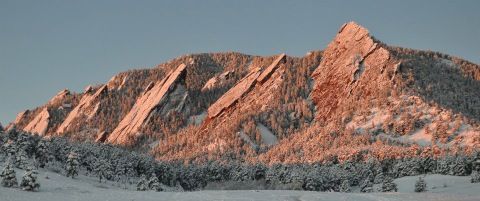
\includegraphics[scale=0.4]{./img/photo1.png}
    \caption{Photo 1}
    \label{fig:p1}
  \end{subfigure}
  \begin{subfigure}{\textwidth}
    \centering
    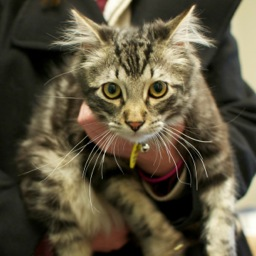
\includegraphics[scale=0.4]{./img/photo2.png}
    \caption{Photo
    2}
    \label{fig:p2}
  \end{subfigure}
  \caption{Provided
  Images}
  \label{fig:init_image}
\end{figure}

